% Chapter Template

\chapter{Modelatge UML de configuracions dels monitors} % Main chapter title

\label{ModelatgeConfiguracions} % Change X to a consecutive number; for referencing this chapter elsewhere, use \ref{ChapterX}


Finalitzada l'especificació de disseny i tècnica dels monitors i les seves configuracions, així com els detalls de la seva implementació, ja tenim definit un sistema de monitoratge que satisfà els criteris d'\textbf{heterogeneïtat} i \textbf{distribució}. Aquestes característiques queden garantides dins el sistema de monitoratge com a unitat independent.\\

El següent pas és gestionar una extensió del sistema que permeti gestionar l'adaptabilitat dels monitors, i concretament que aquesta pugui ser automatitzada, sense necessitat de definir explícitament crides a peticions de reconfiguració al Orchestrator. Tot i que queda fora de l'abast el disseny d'un sistema d'anàlisi i detecció automàtica de reconfiguracions a aplicar (l'equivalent al sistema d'\textbf{A}nàlisi dins el \textit{MAPE-k}), el nostre objectiu és dotar al sistema de monitoratge d'un sistema d'adaptabilitat, que sigui capaç de processar i computar aquestes reconfiguracions.\\

\section{Requisits del modelatge}

Per poder definir els models amb els quals hem de treballar, primer necessitem definir les necessitats del nostre sistema. En termes genèrics, el sistema d'adaptabilitat a dissenyar necessita resoldre la següent problemàtica:\\

\textit{Donada una \textbf{instància} del sistema de monitoratge, el sistema ha de rebre una \textbf{proposta de reconfiguració} dels monitors, basada en la modificació d'una \textbf{característica} específica, aplicant un \textbf{conjunt d'accions} sobre els \textbf{elements del sistema} determinats.}\\

Per major aclariment, anem a analitzar el significat de cadascun dels conceptes introduïts en aquesta definició:

\begin{enumerate}
\item \textbf{Instància del sistema}. Referent al conjunt de \textbf{classes} que defineixen els diferents tipus de configuracions persistents al sistema (és a dir, les diferents implementacions de processos de monitoratge associats a les diferents \textit{tools}), i les \textbf{instàncies} actives corresponents (o processos de monitoratge actius).
\item \textbf{Proposta de reconfiguració}. Necessitem modelar, per una banda, el conjunt de característiques que podem referenciar i editar dins el nostre sistema. Aquestes inclouen, per exemple, la definició de l'atribut \textit{timeSlot} de les instàncies dels monitors de Twitter dins el tipus de monitor SocialNetwork. Per altra banda, necessitem modelar, basat en aquest model de característiques, propostes de configuracions específiques, on es defineixin p.e. valors específics d'aquest \textit{timeSlot}.
\item \textbf{Característica específica}. En relació al punt anterior, que engloba un conjunt de característiques modificables en el sistema, necessitem referenciar quina característica volem modificar.
\item \textbf{Conjunt d'accions}. A partir de les propostes de configuració, i l'aplicació d'una característica específica, hem de definir les diferents accions que s'han de realitzar sobre la instància actual del sistema. Aquestes accions inclouran, seguint amb el mateix exemple, la modificació p.e. d'un atribut com \textit{timeSlot}.
\item \textbf{Elements del sistema}. Necessitem referenciar sobre quins elements del sistema volem aplicar els canvis. És a dir: hem de ser capaços de referenciar, dins el model del sistema, quines instàncies cal modificar i quines no, per tal d'aplicar les accions basades en les característiques anteriors només als que ens interessin.
\end{enumerate}

\section{Disseny de models UML}

Partint d'aquests requisits conceptuals, necessitem definir el conjunt de models amb els quals treballarem per representar tots aquests punts, i permetre així la computació automàtica de canvis dins el nostre sistema. Procedirem presentant cadascun dels models, explicant breument en què consisteixen, i més profundament com s'apliquen al nostre projecte.\\

La implementació i gestió d'aquests models es realitzarà utilitzant l'eina Papyrus, introduïda anteriorment al \textit{Capítol 5. Eines de desenvolupament}. Concretament, pel tractament i gestió de la seva implementació es farà servir la llibreria UML2, versió 5.0.0.

\subsection{Base Model}

Definirem \textit{Base Model} com un diagrama de classes UML que defineix les diferents classes que representen cadascun dels diferents tipus de configuracions de monitors i les seves instàncies. Conceptualment, per tant, és senzill de concebre dins el nostre context, ja que no ve a ser res més que una representació en UML del sistema. D'acord amb el nostre disseny, les necessitats d'aquest disseny UML són les següents: 

\begin{itemize}
\item Cal definir una \textbf{classe abstracta} que representi l'abstracció genèrica de totes les configuracions: és a dir, que englobi aquelles propietats (atributs) compartits entre totes les \textit{tools} del nostre sistema. En el nostre cas, aquests seran: \textit{timeSlot}, \textit{kafkaEndpoint}, \textit{kafkaTopic}, \textit{toolName} i el propi identificador \textit{id}.
\item A continuació cal afegir les implementacions d'aquesta classe abstracta basades en les possibles diferents configuracions que es poden donar d'alta en el nostre sistema. En definitiva: totes aquelles varietats de configuracions segons els diferents paràmetres a definir (que en el nostre sistema ve a ser equivalent a les diferències entre tipus de monitors).
\item Per cadascuna d'aquestes implementacions, cal modelar el conjunt de configuracions (és a dir, instàncies de classes), amb els valors dels atributs definits.
\end{itemize}

\begin{figure}
\centering
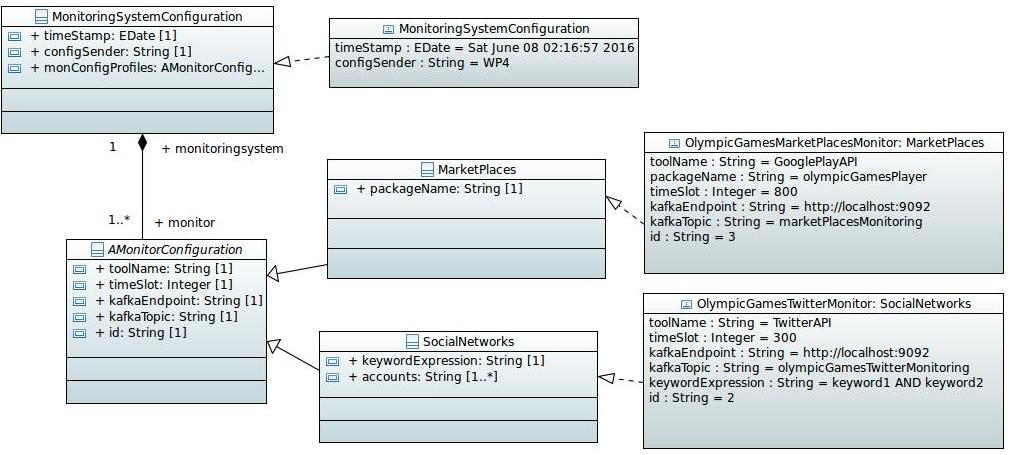
\includegraphics[width=13cm]{Figures/Figure16}
\decoRule
\caption{Exemple de Base Model del sistema de monitoratge}
\label{fig:Figura16}
\end{figure}

A la figura ~\ref{fig:Figura16} podem visualitzar un exemple de \textit{Base Model} que representa aquesta fotografia d'un sistema on tenim definits el monitor de Twitter i el de Google Play. \textit{AMonitorConfiguration} representa la classe abstracta dels diferents tipus de configuracions; \textit{SocialNetworks} i \textit{MarketPlaces} representen les extensions de configuracions genèriques amb els paràmetres addicionals definits; i finalment, \textit{OlympicGamesMarketPlacesMonitor} i \textit{OlympicGamesTwitterMonitor} són instàncies dels diferents tipus de configuracions (no s'ha afegit el monitor d'AppStore per simplicitat en l'exemplificació). També veiem addicionalment una classe anomenada \textit{MonitoringSystemConfiguration}, en relació d'agregació a \textit{AMonitorConfiguration}, i una instància d'aquesta mateixa. Aquestes són classes establertes com a requisits dins el context SUPERSEDE, i per tant no són necessàries a tenir en compte.\\

L'objectiu principal de l'adaptabilitat del sistema serà aplicar canvis en aquest \textit{Base Model} que defineix l'estat actual del sistema. Així, el sistema d'adaptabilitat actualitzarà per una banda el \textit{Base Model} actual, aplicant els canvis pertinents, i computarà les diferències amb l'anterior per definir reconfiguracions que s'enviaran al Orchestrator.

\subsection{Features}

Aquests canvis, que anomenem de forma genèrica, són modificacions dins el diagrama de classes del sistema, i per tant inclou aspectes com la modificació del valor d'un atribut d'una instància de configuració. Però aquestes modificacions no poden ser aleatòries: suposant que no considerem el comportament del sistema de \textit{\textbf{P}lanificació} dins el \textit{MAPE-k}, i per tant no definim l'autogeneració de noves propostes de configuracions del sistema, necessitem modelar de forma definida una sèrie de casos, o configuracions predefinides, que defineixin un \textbf{conjunt de combinacions de característiques} adreçades a aplicar-se en diferents casos. És a dir: necessitem modelar d'alguna forma diferents alternatives per valors dels diferents atributs de les configuracions.\\
 
En termes específics, el que estarem fent serà definir un conjunt de propostes que aplicarem per a casos específics. Podríem, per exemple, modelar una proposta de configuració que disminueixi el valor del \textit{timeSlot} quan el volum de dades obtingudes pel monitoratge sigui molt baix, i vulguem rebre aquestes amb menys periodicitat; o bé podríem re-orientar les dades a un \textit{kafkaEndpoint} diferent quan, per diferents motius, el \textit{kafkaEndpoint} actual estigui caigut i les dades rebotin. Davant aquests exemples, i un nombre indeterminat (d'acord amb les nostres necessitats), podem definir diferents casos o propostes que representin semànticament un canvi en el sistema.\\

Per modelar aquest aspecte, introduïm dos tipus de models addicionals: el \textbf{\textit{Feature Model}} i les \textbf{\textit{Feature Configurations}}.

\subsubsection{Feature Model}

Un \textit{Feature Model} (FM), o model de característiques, en la seva definició genèrica, és un diagrama que permet gestionar el conjunt d'aspectes comuns i variables dins d'un sistema i els seus components. Representa, en definitiva, una modelització estandarditzada que defineix una jerarquia entre aquestes característiques i estableix les diferents opcionalitats de configuració dins un sistema.\\

\begin{figure}
\centering
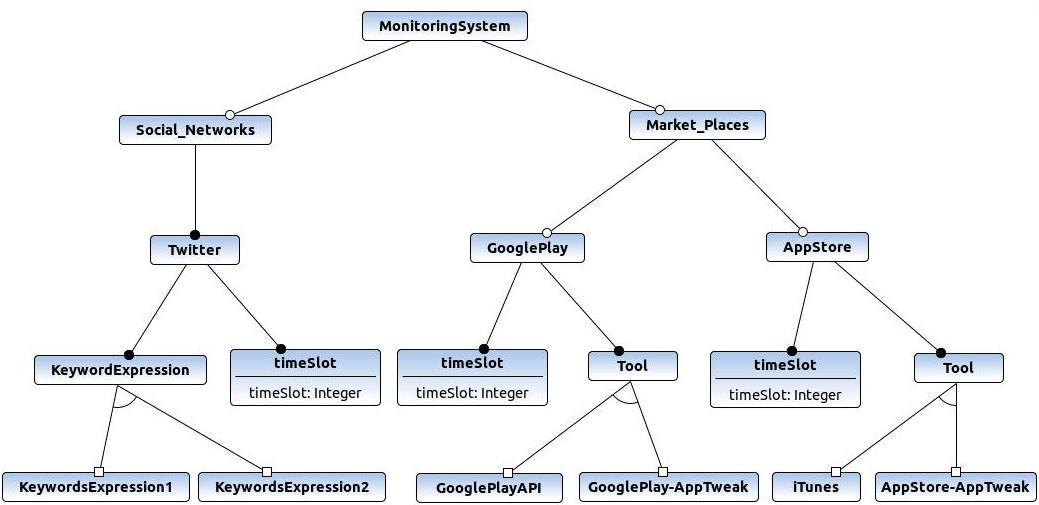
\includegraphics[width=14cm]{Figures/Figure17}
\decoRule
\caption{Exemple de Feature Model del sistema de monitoratge}
\label{fig:Figura17}
\end{figure}

Aplicat al nostre context, un \textit{Feature Model} ens serveix per definir quines característiques del nostre sistema podem referenciar i modificar, i com s'estructuren aquestes des d'un punt de vista jeràrquic d'acord amb les implementacions de la classe abstracta de configuració de monitors. Un dels casos d'ús que contemplarem, ja que permet validar el nostre sistema alhora que mostrar fàcilment la repercussió dels canvis, és la reconfiguració de l'atribut \textit{timeSlot} d'una instància de monitor. A la figura ~\ref{fig:Figura17} podem observar un exemple de \textit{Feature Model} del nostre sistema. Com podem veure, representa una modelació conceptual del sistema de monitoratge i la seva jerarquia: un sistema de monitoratge, amb el conjunt de tipus de monitors, que implementen un conjunt de monitors específics, on cadascun d'ells engloben una sèrie de \textit{features}, és a dir, característiques que podem referenciar del nostre sistema. En aquest exemple, si ens fixem per exemple en el cas de Twitter, tenim per una banda la \textit{feature} \textit{timeSlot}, representada com un Integer de valor variable, i \textit{keywordExpression}, que en comptes de tenir un valor (com podria ser un string) editable, defineix dues característiques opcionals, que representen dos possibilitats de valor associades a aquesta \textit{feature}. De manera similar trobem el cas del monitor de Google Play i d'App Store, on la \textit{feature} \textit{toolName} és només configurable amb dos opcions en cada cas, segons les \textit{tools} que tenen implementades, i de nou el \textit{timeSlot}. Cal destacar que aquest es tracta únicament d'un exemple de \textit{Feature Model}: les diferents \textit{features} es podrien ampliar i/o modificar, p.e. afegint noves \textit{tools} conforme s'implementin, o bé afegint altres paràmetres a modificar (p.e. \textit{kafkaEndpoint} o \textit{kafkaTopic}).

\subsubsection{Feature Configuration}

Una \textit{Feature Configuration} (FC) representa una configuració específica d'un \textit{Feature Model}. És a dir: davant les diferents opcionalitats i variabilitats que un \textit{Feature Model} defineix, com poden ser la personalització del valor d'una \textit{feature}, o bé la selecció entre un conjunt d'opcions, la \textit{Feature Configuration} és la modelació d'un cas específic d'aquestes \textit{features}. A diferència del \textit{Feature Model}, que presenta totes les opcions del sistema, la \textit{Feature Configuration} presenta només una opció específica per aquells punts variables dins el \textit{Feature Model}. Aquestes opcions específiques reben el nom de \textbf{selections} (seleccions).\\

Aplicat al nostre context, i seguint amb l'exemple anterior, l'objectiu d'una \textit{Feature Configuration} es modelar una proposta de configuració del sistema de monitoratge. Així, definim uns valors específics pels atributs de les configuracions. A la figura ~\ref{fig:Figura18} podem visualitzar un exemple basat en el \textit{Feature Model} de la figura ~\ref{fig:Figura17}.\\

\begin{figure}
\centering
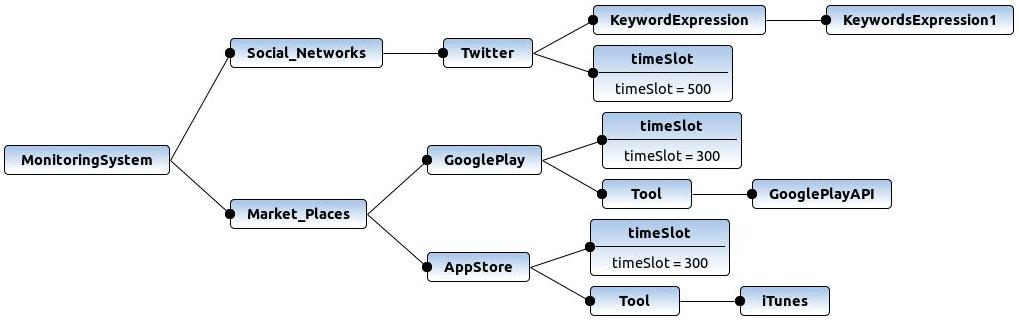
\includegraphics[width=13cm]{Figures/Figure18}
\decoRule
\caption{Exemple de Feature Configuration del sistema de monitoratge}
\label{fig:Figura18}
\end{figure}

Si ens fixem en aquesta \textit{Feature Configuration} i la comparem amb el \textit{Feature Model}, veiem que tots els punts de variabilitat que aquesta segona definia s'especifiquen amb un valor o opcions específics. Per aquest cas, p.e., es proposa un valor de timeSlot específic per les configuracions de tots els tipus de monitors; paral·lelament, en el cas del monitor de Twitter s'especifica la \textit{KeywordExpression1} com a opció a triar per aquest paràmetre, i les tools de \textit{GooglePlayAPI} i \textit{iTunes} per les \textit{tools} dels monitors de Market Places. En definitiva, és la representació d'una proposta de configuració de les \textit{features} definides. Orientat al nostre cas d'ús, aquesta proposta ens permet traduir-les al \textit{Base Model} en una sèrie de modificacions d'atributs.\\

\subsection{Advice Model}

En alguns casos, i especialment considerant l'expansió i futur treball a partir de les bases establertes per aquest projecte, la modificació de models pot anar més enllà de la modificació o actualització d'un valor com el \textit{timeslot} o algun altre paràmetre, com hem plantejat abans. De fet, per assolir una autonomia total del sistema de monitoratge, aquest hauria de ser capaç de modificar completament la seva activitat, mitjançant p.e. l'alta de nous processos de monitoratge o l'eliminació de processos existents.\\

Per aquest motiu, tot i que no serà el cas d'estudi d'aquest projecte, cal introduir el concepte d'\textit{Advice Model}. Aquests models seran, dins el nostre context, diagrames de classes i instàncies en UML que modelen una secció del nostre sistema, com per exemple noves configuracions per a un monitor. La seva característica principal és que, a diferència dels \textit{Base Model}, que representen una modelació d'un estat del sistema, aquests defineixen variacions, punts de variabilitat que es poden afegir, eliminar o substituir al \textit{Base Model} original (més endavant veurem en què consisteixen aquestes modificacions). A la figura ~\ref{fig:advice} podem veure un exemple aplicable al nostre context: una representació de dues propostes de noves configuracions de monitoratge que es podrien afegir al sistema.

\subsection{Pattern Model}

Aquesta modificació d'atributs, però, únicament ens està definint una acció genèrica. És a dir, la semàntica que podem desprendre d'una \textit{Feature Configuration} és simplement la definició d'una proposta general per les configuracions dels monitors. El problema, però, està en que la \textit{Feature Configuration} defineix tot el conjunt del sistema (en aquest cas, tots els atributs de tots els monitors), però no ens dona cap informació sobre quines instàncies del \textit{Base Model} cal aplicar aquests canvis. És a dir: suposem que al \textit{Base Model} de la figura ~\ref{fig:Figura16} volem actualitzar el \textit{timeSlot} de la instància \textit{OlympicGamesTwitterMonitor}, però no de la instància \textit{OlympicGamesMarketPlacesMonitor}.\\

Amb aquest objectiu, necessitem afegir informació addicional, una forma de modelar la identificació dels elements sobre els quals volem aplicar els canvis de reconfiguració (aplicant criteris variats, segons cada cas). Per satisfer aquesta necessitat, utilitzarem els \textit{Pattern Models}. Aquests models defineixen, mitjançant un llenguatge específic de la llibreria UML2 (\textit{Viatra Query Language}, VQL), patrons de cerca que permeten retornar elements (classes, instàncies, relacions, atributs, etc.) dins un diagrama UML.\\ 

\begin{figure}
\centering
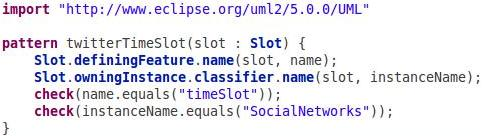
\includegraphics[width=11cm]{Figures/Figure19}
\decoRule
\caption{Exemple de Pattern Model del sistema de monitoratge}
\label{fig:Figura19}
\end{figure}

A la figura ~\ref{fig:Figura19} podem veure un exemple de \textit{Pattern} aplicat al nostre cas d'estudi. Sense entrar en els detalls específics de la sintaxi, aquest patró anomenat \textit{twitterTimeSlot} retorna tots els objectes de tipus \textit{Slot}, que en l'especificació UML2 venen a ser els atributs d'una instància d'una classe, que compleixen dues característiques: que reben per nom \textit{timeSlot} (1) i que són atributs d'una instància de la classe amb nom \textit{twitter} (2). Així, quan vulguem aplicar de forma dinàmica adaptacions sobre el sistema, i concretament sobre els \textit{timeSlots} (1) de les instàncies de monitoratge del monitor de Twitter (2), podem referenciar aquests objectes amb la màxima eficiència, utilitzant les eines que la pròpia llibreria ens dona per treballar dinàmicament amb models UML.\\

De manera similar a les FC, necessitarem definir un \textit{pattern} diferent per cada cas d'adaptació, d'acord amb els criteris específics. Tot i que això no exclou que alguns siguin reutilitzables entre diferents reconfiguracions. El potencial del VQL ens permet generar, amb una sintaxi relativament senzilla, patrons de cerca de tot tipus i que filtrin la cerca segons tot tipus de criteris: valors dels atributs de les instàncies, tipus de configuracions, relacions amb superclasses, etc. 
 
\subsection{Profile Model}

A partir dels \textit{patterns} definits, som capaços d'obtenir i referenciar aquests objectes UML sobre els quals aplicar adaptacions. Un cop obtinguts, a aquests elements se'ls aplica un rol o \textit{stereotype} específic, que ens servirà bàsicament per distingir entre diferents tipus d'adaptacions dins d'una mateixa adaptació. És a dir: suposem que, dins una mateixa adaptació, volem actualitzar per una banda les configuracions dels processos de monitoratge del monitor de Twitter amb un valor \textit{x} i, per altra banda, les del monitor de GooglePlay amb un valor \textit{y}. Un cop l'Adapter computi les adaptacions i obtingui els elements a adaptar, es comunicarà amb el Model Adapter per sol·licitar-li l'aplicació d'una acció sobre els elements trobats identificats amb un rol específic. Aquesta adaptació composta queda fora del nostre abast, però és important introduïr per entendre el disseny genèric dels nostres models d'adaptació. Per la tasca d'etiquetar models, utilitzarem els anomenats \textit{Profile Models}, que són models que defineixen una classificació de rols o \textit{stereotypes} a aplicar sobre un cert grup d'elements UML segon el seu tipus i les seves característiques.\\

Pel nostre context, simplement identificarem un \textit{stereotype} que anomenarem \textit{jointpoint}, i ens servirà per etiquetar, dins el \textit{Base Model}, aquells elements (bàsicament, \textit{slots}) que requereixen ser actualitzats. A la figura ~\ref{fig:profile} podem veure el \textit{Profile Model} utilitzat a SUPERSEDE per l'adaptació de models. No ens centrarem en la seva sintaxi a fons; únicament ens centrarem en el rol \textit{jointpoint}, que segons modela el \textit{Profile Model}, pot ser aplicat a qualsevol objecte UML que implementi \textit{Element} (que, segons la documentació de UML2, són tots aquells elements del diagram UML).\\

\begin{figure}
\centering
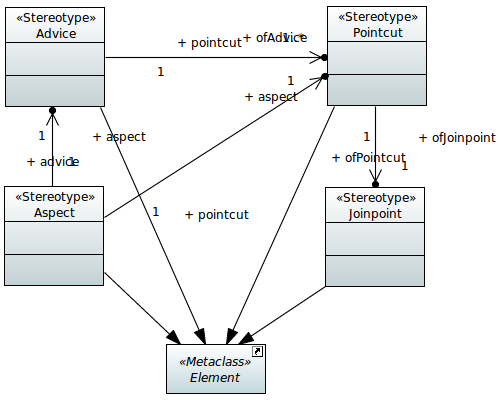
\includegraphics[width=11cm]{Figures/profile}
\decoRule
\caption{Exemple de Profile Model del sistema de monitoratge}
\label{fig:profile}
\end{figure}

\subsection{Aspect Model}

Aquest tipus de model es tracta d'un tipus de document dissenyat i implementat per \textit{partners} del projecte SUPERSEDE. Com a tal, el projecte inclou una llibreria capaç de processar i interpretar dinàmicament aquest model i les seves referències. Ens referirem a ell com a \textit{Aspect Model} o \textit{Adaptability Model}, ja que bàsicament es tracta d'un fitxer de format similar a un JSON que, des d'un punt de vista semàntic, descriu adaptacions específiques interrelacionant els elements que intervenen en una adaptació del sistema. Aquests aspectes inclouen:

\begin{itemize}
\item \textbf{FeatureId}. Referencia la \textit{feature} d'un \textit{Feature Model} sobre la qual descriu una adaptació específica.
\item \textbf{Pointucts}. Llistat de punts on s'han d'aplicar canvis per aquella reconfiguració. Per cada \textit{pointcut} que definim, s'especifica:
\begin{itemize}
\item \textbf{Pattern}. El \textit{pattern} utilitzat per buscar dinàmicament els elements al diagrama UML
\item \textbf{Role}. El rol o \textit{stereotype} amb el qual s'etiquetaran aquests elements
\end{itemize} 
\item \textbf{Compositions}. Llistat de les adaptacions a realitzar sobre els punts o elements anteriorment identificats. Per cada \textit{composition} que definim, s'especifica:
\begin{itemize}
\item \textbf{Feature enabled}. Indica si s'ha d'aplicar quan la \textit{Feature Configuration} indica que aquella \textit{feature} passa a estar activada o desactivada
\item \textbf{Jointpoint role}. Indica el rol que han de tenir els elements sobre els quals s'han d'aplicar el canvi definit per aquesta \textit{composition}. En aquest punt entraria en joc la composició d'adaptacions introduïda anteriorment al explicar els \textit{Profile Models}.
\item \textbf{Action}. Indica el tipus d'acció a aplicar. En distingirem 2 tipus:
\begin{itemize}
\item \textbf{Update}. Serà la operació en la qual ens centrarem per validar el nostre sistema. Consisteix en actualitzar el valor d'un atribut (\textit{slot} en termes de modelació en UML2)
\item \textbf{Add/Delete/Replace}. Tot i que queden fora de l'abast de validació del nostre projecte, les afegirem al disseny i desenvolupament del projecte davant les necessitats del desenvolupament a SUPERSEDE. Es tracta d'operacions que, en referència a un \textit{Advice Model} afegeixen, eliminen o substitueixen els elements UML presents a l'\textit{Advice Model} al punt d'injecció definit com a \textit{jointpoint} al \textit{Base Model}.
\end{itemize}
\end{itemize}
\end{itemize}

A la figura ~\ref{fig:aspect} podem veure un exemple de model d'adaptabilitat amb els paràmetres anteriorment definits. En aquest cas, l'operació a aplicar és \textit{Update}, ja que serà la que ens interessarà pel cas d'estudi.

Aquesta es tracta d'una aproximació genèrica inicial als models d'adaptabilitat. Per entendre el seu funcionament exacte i aprofundir en la sintaxi i les seves implicacions, en el següent capítol descriurem l'algorisme d'adaptabilitat i reconfiguració de monitors per entendre precisament com aquesta adaptació funciona amb els nostres models.\\

\begin{figure}
\centering
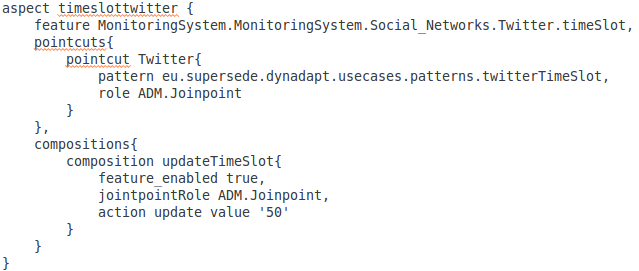
\includegraphics[width=11cm]{Figures/Figure38}
\decoRule
\caption{Exemple de Pattern Model del sistema de monitoratge}
\label{fig:aspect}
\end{figure}